% MDPI-style working manuscript package; generated from frozen Markdown at Git ad00fb0.
\documentclass[technologies,article,submit,moreauthors]{Definitions/mdpi}

% The official class expects publication metadata commands in its example template.
% These fields are intentionally left blank because no journal/publication metadata is approved.
\makeatletter
\gdef\@pubvolume{0}
\gdef\@issuenum{0}
\gdef\@articlenumber{0}
\gdef\@pubyear{}
\gdef\@copyrightyear{}
\makeatother
\firstpage{1}
\datereceived{}
\daterevised{}
\dateaccepted{}
\datepublished{}
\setlength{\headheight}{20pt}

% The generic submit-mode class synthesizes a DOI from volume/issue/article fields.
% No DOI is assigned, so suppress only that unassigned DOI footer.
\fancyfoot[R]{}
\fancypagestyle{plain}{%
  \fancyhf{}%
  \fancyhead{\null\vspace{8pt}}%
  \renewcommand{\footrulewidth}{0.4pt}%
  \fancyfoot[L]{\fontsize{8}{8}\selectfont Version \today\ submitted to \emph{\journalname}}%
  \fancyfoot[R]{}%
}

% Final title and keywords confirmed by the author on 2026-10-20.
% Author identities, order, and affiliations were supplied by the author and
% updated on 2026-10-20. Corresponding authors: Vassiliy Serbin and Aray Kassenkhan.
\newcommand{\PaperTitle}{Profile Poisoning and Selective-Update Bias in Online Behavioral Biometric Authentication}
\newcommand{\orcidauthorA}{0009-0006-2621-0454}
\newcommand{\orcidauthorB}{0000-0002-5807-3873}
\newcommand{\orcidauthorC}{0000-0002-6355-9544}
\newcommand{\orcidauthorD}{0000-0003-1042-1530}
\newcommand{\orcidauthorE}{0000-0003-0716-5265}
\newcommand{\orcidauthorF}{0009-0002-4089-9332}
\newcommand{\orcidauthorG}{0009-0009-8985-5892}
\newcommand{\PaperAuthors}{Madi Gali $^{1}$\orcidA{}, Vassiliy Serbin $^{2,*}$\orcidB{}, Aray Kassenkhan $^{3,*}$\orcidC{}, Aliya Turegeldinova $^{4}$\orcidD{}, Bakytzhan Amralinova $^{5}$\orcidE{}, Shyndauyl Nugumanov $^{5}$\orcidF{} and Yersain Chinibayev $^{3}$\orcidG{}}
\newcommand{\PaperAuthorNames}{Madi Gali, Vassiliy Serbin, Aray Kassenkhan, Aliya Turegeldinova, Bakytzhan Amralinova, Shyndauyl Nugumanov and Yersain Chinibayev}
\newcommand{\PaperAffiliations}{%
$^{1}$ \quad Department of Cybersecurity, Institute of Automation and Information Technologies, Satbayev University, Almaty 050013, Kazakhstan; \href{mailto:gali.m@stud.satbayev.university}{gali.m@stud.satbayev.university}\\
$^{2}$ \quad Department of Information Systems, Institute of Automation and Information Technologies, Satbayev University, Almaty 050013, Kazakhstan; \href{mailto:v.serbin@satbayev.university}{v.serbin@satbayev.university}\\
$^{3}$ \quad Department of Software Engineering, Institute of Automation and Information Technologies, Satbayev University, Almaty 050013, Kazakhstan; \href{mailto:a.kassenkhan@satbayev.university}{a.kassenkhan@satbayev.university} (A.K.); \href{mailto:y.chinibayev@satbayev.university}{y.chinibayev@satbayev.university} (Y.C.)\\
$^{4}$ \quad Department of Management and Mathematical Economics, Satbayev University, Almaty, Kazakhstan; \href{mailto:a.turegeldinova@satbayev.university}{a.turegeldinova@satbayev.university}\\
$^{5}$ \quad Project Management Institute, Satbayev University, Almaty, Kazakhstan; \href{mailto:b.amralinova@satbayev.university}{b.amralinova@satbayev.university} (B.A.); \href{mailto:s.nugumanov@satbayev.university}{s.nugumanov@satbayev.university} (S.N.)
}
\newcommand{\PaperCorrespondence}{Correspondence: \href{mailto:v.serbin@satbayev.university}{v.serbin@satbayev.university} (V.S.); \href{mailto:a.kassenkhan@satbayev.university}{a.kassenkhan@satbayev.university} (A.K.)}
\newcommand{\PaperKeywords}{behavioral biometrics; continuous authentication; template update; online adaptation; profile poisoning; selective-update bias; mobile security; adversarial machine learning}
\newcommand{\PaperAbstract}{Behavioral continuous authentication can update a user's profile during operation, but accepted-only adaptation links access errors to future model state. Prior biometric work established separate authentication and update thresholds and quantified erroneous impostor inclusion and genuine-update misses. We examine their coupled security and adaptation consequences in score-level mobile authentication using frozen HMOG long short-term memory scores, a synthetic feature-space shift, and an independent two-day McGill Gait protocol. Poisoning samples were separated from future impostor probes. The strongest benchmark assumed access to claimant scores and presented up to eight initially accepted samples ranked near the authentication boundary; reconnaissance and candidate screening were not counted. At the reference operating points, Blind exponential moving-average (EMA) updating increased post-poison attack success rate from 22.92\% to 53.96\% on HMOG and from 12.37\% to 32.09\% on McGill. An enrollment-anchored Guarded EMA condition kept the reference-point result close to Frozen. This direction did not persist across recalibrated policies. Under the nominal-1\% calibration condition, the mean Blind-minus-Frozen effect was negative on both datasets for the tested boundary strategy. On the same HMOG conditional cohort, Blind EMA reduced attack success by 0.447 percentage points but increased false rejection by 6.89 points and half total error rate by 3.22 points. Full-cohort false rejection at this strict condition was 80.79\% on HMOG and 90.25\% on McGill. The Guarded rule added no update margin when the current authentication threshold reached or exceeded the enrollment mean. In separate temporal evaluations, Guarded did not improve late genuine acceptance relative to Frozen. A label-aware, non-deployable Oracle-all diagnostic changed profile trajectories and reduced false rejection, but increased false acceptance. The results show that poisoning effects, genuine rejection, update-gate activity, calibration transfer, and attack feasibility depend on the operating point and should be evaluated together.}

\Title{\PaperTitle}
\Author{\PaperAuthors}
\AuthorNames{\PaperAuthorNames}
\address{\PaperAffiliations}
\corres{\PaperCorrespondence}
\abstract{\PaperAbstract}
\keyword{\PaperKeywords}

\begin{document}

\section{Introduction}\label{sec:introduction}

Initial login verifies the operator at one moment. Continuous behavioral authentication instead estimates identity throughout a device session from signals such as touch, keystroke, gait, and hand motion \cite{Mahfouz2017SmartphoneSurvey,Abuhamad2021SensorSurvey,Stylios2021MobileSurvey}. Smartphone studies have shown that interaction and inertial measurements can provide repeated identity evidence without requiring an explicit biometric action for every decision \cite{Frank2013Touchalytics,Sitova2016HMOG,Fereidooni2023AuthentiSense}. The same evidence varies across sessions, activities, device placement, acquisition conditions, and time. A profile fixed at enrollment may therefore become less representative of its user.

Online updating can follow this variation, but it must obtain trustworthy update labels. Unsupervised biometric systems commonly infer them from the current matcher \cite{Rattani2009TemplateUpdate,Didaci2014UnsupervisedUpdate}. An accepted impostor can then alter the profile used for later decisions, a risk already demonstrated in adaptive face and fingerprint systems \cite{Biggio2012PoisoningAdaptive,Biggio2013FacePoisoning,Lovisotto2020BiometricBackdoors,Xue2020LOPA}. Requiring acceptance before learning also removes rejected genuine observations from the adaptive stream. During a downward genuine-score shift, the updater retains higher-scoring samples and loses observations that indicate a need for recovery. Selective-label and self-training research provides analogous context for this decision-conditioned evidence problem \cite{Lakkaraju2017SelectiveLabels,Arazo2020ConfirmationBias,Perdomo2020PerformativePrediction}. We call the authentication-specific mechanism \emph{selective-update bias caused by accepted-only feedback censoring}.

Separate authentication and update thresholds, erroneous impostor inclusion, and missed genuine updates have been studied directly in behavioral template update \cite{Giot2011KeystrokeUpdate,Giot2012HybridTemplateUpdate,Giot2012TemplateUpdateEvaluation}. Deliberate poisoning of self-updating biometrics is also established prior art \cite{Biggio2012PoisoningAdaptive,Biggio2013FacePoisoning,Lovisotto2020BiometricBackdoors,Xue2020LOPA}. The open question addressed here is their coupled, operating-point-dependent effect in mobile behavioral authentication: how admitted malicious samples affect unused future probes, how conservative update eligibility changes genuine evidence, and whether these relationships persist under recalibration and a second dataset. Reviews of adaptive biometrics report limited continuous-mobile and longitudinal evaluation, while our prior systematic review found limited standardized adversarial and longitudinal evidence within its searched corpus \cite{Ryu2023AdaptiveBiometrics,Gali2026SystematicReview}. The study is therefore positioned as a bounded mechanism analysis rather than a new two-threshold algorithm, a new update-error metric family, or a first biometric poisoning attack.

The present work studies malicious inclusion and genuine-evidence censoring in one experimental framework. Our previous HMOG study used a fixed long short-term memory (LSTM) score generator and an accepted-only exponential moving-average (EMA) profile; EMA did not improve half total error rate over a frozen threshold, and its label-blind update path could admit an accepted impostor \cite{Serbin2026AdaptiveLSTM}. That study did not run a dedicated poisoning experiment. Here, random and score-informed boundary attacks use poisoning observations separated from held-out future probes. The boundary benchmark assumes claimant-score access and ranks samples accepted near the initial threshold. Its budget counts selected poisoning presentations, not reconnaissance or screening, so it is not an eight-query or binary-feedback-only attack.

This design asks whether state change affects observations that were not used to choose the attack. It also keeps access evaluation separate from learning eligibility, allowing malicious incorporation, genuine update availability, and later error rates to be reported as distinct quantities.

We compare Frozen, Blind EMA, an enrollment-anchored Guarded EMA update condition, and label-aware Oracle controls. Guarded retains the access-decision rule form but changes update eligibility; its update history can therefore change later state, thresholds, and decisions. Oracle-all admits every ground-truth genuine adaptation observation to diagnose the information removed by accepted-only updating. It is not deployable or a formal performance upper bound. HMOG temporal experiments use a controlled synthetic feature-space shift with adaptation observations separated from evaluation checkpoints. A two-day McGill Gait protocol provides independent cross-day corroboration, although day separation does not isolate behavioral drift from acquisition and model-transfer effects \cite{Frank2010McGillGaitDataset}.

The study makes three contributions:

\begin{enumerate}
\def\labelenumi{\arabic{enumi}.}
\item
  It pairs fixed-score profile updating on separated poisoning and future-probe observations, with explicit update eligibility and diagnostic temporal controls.
\item
  It quantifies operating-point-specific changes in attack effect, feasible paths, gate activity, genuine rejection, and calibration transfer.
\item
  It tests whether these coupled relationships recur under the documented McGill policy and explains a local EMA boundary transition, while limiting generalization to the evaluated protocols.
\end{enumerate}

The recovery-state and quantile-profile branches test alternative explanations but are not headline methods. TQ-EMA v1 reached outer evaluation without meeting its recovery criterion. TQ-EMA v2 and the Quantile branch failed their validation gates, and their outer outcomes were not loaded. Reporting these stops preserves the development evidence without treating unsuccessful variants as contributions.

The historical HMOG reference threshold was approximately equal-error, while McGill used minimum Day-1 half total error. Sensitivity conditions targeted 5\% and 1\% calibration false acceptance, not guaranteed held-out rates or deployment standards. Recalibration changed the initial threshold, its associated profile coefficient, the selected boundary candidates, and the feasible attack cohort. Accordingly, neither Guarded performance at the reference points nor a negative mean attack-success effect at the strict point establishes general security. Recovery and quantile branches are retained as supporting negative probes rather than algorithmic contributions.

\section{Related Work}\label{sec:related-work}

\subsection{Mobile behavioral authentication}\label{sec:mobile-behavioral-authentication}

Continuous mobile authentication has used touch and swipe dynamics, keystroke behavior, gait, hand motion, contextual signals, and multimodal combinations \cite{Mahfouz2017SmartphoneSurvey,Abuhamad2021SensorSurvey,Stylios2021MobileSurvey}. Touchalytics reported distinct intra-session, inter-session, and delayed behavior \cite{Frank2013Touchalytics}. SilentSense combined touch with device movement, while HMOG derived hand-movement, orientation, and grasp features from inertial and interaction data \cite{Bo2013SilentSense,Sitova2016HMOG}. Recent systems combine motion, touch, and usage context or learn identity from inertial streams \cite{Shen2022MMAuth,Fereidooni2023AuthentiSense,Jiang2024MAUTH}. These studies establish that mobile behavior carries identity information and that its availability and distribution vary with context.

Modalities also differ in when they produce evidence. Touch and keystroke observations depend on particular actions, whereas inertial streams can reflect gait, posture, or device handling over a broader set of activities. Multimodal systems can compensate for missing signals but introduce fusion, calibration, and resource decisions \cite{Ross2003InformationFusion,Shen2022MMAuth}. These differences matter for adaptation because an update policy observes only the modalities and contexts present at that moment.

The primary dataset in this study is HMOG. McGill supplies a different temporal setting: its official archive contains smartphone gait recordings from 20 individuals on two collection days \cite{Frank2010McGillGaitDataset,Frank2010ActivityGait}. McGill and HMOG differ in population, sensors, activity, classifier, and chronology, so their absolute error rates are not treated as benchmark comparisons. McGill is used to test whether the reference mechanisms recur after Day-1 development and Day-2 evaluation.

Other gait studies provide attack and unconstrained-collection context rather than interchangeable baselines. Live imitation has been studied against smartphone gait authentication, and whuGAIT was developed for less constrained smartphone collection \cite{Muaaz2017GaitImitation,Zou2020WhuGait}. The archive inspected for this project did not preserve the chronology needed for the unified temporal protocol, so it was not used as an experimental dataset.

\subsection{Adaptive profiles and poisoning}\label{sec:adaptive-profiles-and-poisoning}

Template update addresses ageing and intra-class variation by revising a biometric reference after enrollment. Supervised methods use externally verified labels; semi-supervised and unsupervised methods reuse matcher decisions \cite{Rattani2009TemplateUpdate,Didaci2014UnsupervisedUpdate}. Behavioral work has applied adaptation to multi-session keystrokes and accelerometer streams \cite{Giot2011KeystrokeUpdate,Pisani2017AccelerometerAdaptation}. Giot et al.~used separate acceptance and update thresholds and later formalized two complementary self-update errors: the Impostor Update Selection Rate, \(U_i/N_i\), and Genuine Update Miss Rate, \((N_g-U_g)/N_g\), in a multi-gallery keystroke updater \cite{Giot2012HybridTemplateUpdate}. Their evaluation work further showed that temporal aggregation choices can change the interpretation of the same adaptive score sequence \cite{Giot2012TemplateUpdateEvaluation}. Thus, separating access from learning and measuring impostor inclusion or genuine-update omission are established prior art. The Guarded condition here is an experimental intervention for measuring those consequences under held-out poisoning and temporal change.

The source of trust separates these approaches. Supervised update assumes a verified genuine identity. Self-update treats matcher confidence as a proxy label, sometimes requiring a higher threshold or accumulating a batch before changing the reference. Those choices affect both erroneous inclusion and the range of genuine samples visible to the updater. A recent review organizes confidence gates, query acceptance, retraining, and structural adaptation while noting limited continuous-mobile and large-scale longitudinal evidence \cite{Ryu2023AdaptiveBiometrics}.

Self-update transfers recognition errors into future state. Giot et al.~evaluated mixed genuine/impostor streams and update-selection errors rather than attacker-ranked poisoning followed by evaluation on an unused probe pool \cite{Giot2012HybridTemplateUpdate}. Biggio et al.~formalized deliberate poisoning in adaptive biometrics and evaluated face-template compromise \cite{Biggio2012PoisoningAdaptive,Biggio2013FacePoisoning}. Lovisotto et al.~constructed intermediate face samples that exploited unsupervised update, and Xue et al.~attacked online self-updating fingerprint authentication \cite{Lovisotto2020BiometricBackdoors,Xue2020LOPA}. These studies are direct precedents. The present attack is narrower: it does not modify classifier weights, enrollment data, sensor firmware, or raw templates. It presents impostor observations to a score-profile updater and measures later acceptance on unused probes after the state is frozen. The score-informed boundary strategy is a strong benchmark, not a demonstrated binary-feedback search procedure.

Presentation and imitation attacks address a different point in the pipeline. Smartphone gait, for example, has been tested against live mimicry at decision time \cite{Muaaz2017GaitImitation}. Such work evaluates whether an input evades a matcher immediately. Profile poisoning asks whether an accepted input changes state and affects later observations. Broader template-security surveys cover update-related and non-update threats, but direct poisoning claims here rely on the adaptive face and fingerprint studies above \cite{Baaqeel2022AdaptiveSpoofingSurvey,Abdullahi2024TemplateAttacks}.

General online-learning work also studies sequential contamination \cite{Zhang2020OnlinePoisoning}. Its learners and attacker interfaces differ from biometric authentication, so it provides conceptual context rather than direct evidence for the present score profile.

Prior poisoning studies often optimize a sequence for a particular template or matcher. The boundary benchmark here instead selects already accepted scores near the initial profile threshold and then freezes the resulting state before future evaluation. This simpler construction supports matched analysis of update policy and operating point, while leaving stronger adaptive or query-limited attackers untested.

\subsection{Decision-conditioned feedback}\label{sec:decision-conditioned-feedback}

Adaptive-biometric research has already recognized both erroneous inclusion and failure to select genuine observations for update \cite{Giot2012HybridTemplateUpdate}. Selective-label research studies decisions that determine which outcomes become observable; pseudo-labeling research shows how model-assigned labels can reinforce error; performative-prediction theory considers deployed decisions that alter later data \cite{Lakkaraju2017SelectiveLabels,Arazo2020ConfirmationBias,Perdomo2020PerformativePrediction}. Accepted-only authentication differs from each setting. The genuine/impostor label is unavailable to the deployed updater, and the access result controls update eligibility rather than the claimant's underlying behavior. The term \emph{selective-update bias caused by accepted-only feedback censoring} is therefore used here as a scoped description of the observed trajectory mechanism, not as a claim that genuine-update omission was first identified here.

Oracle-all is designed to reveal this information difference. It retains the authentication decision-rule form while authorizing updates from every ground-truth genuine adaptation observation. The resulting state and threshold can change subsequent decisions. Oracle-all is label-aware and non-deployable, and its result does not identify a safe recovery mechanism.

This diagnostic also differs from supervised template update. Ground-truth labels are supplied retrospectively by the experiment, not by an operational identity-verification channel. Oracle-all therefore measures sensitivity to information availability while bypassing the central trust problem that a deployable updater must solve.

\subsection{Position of this study}\label{sec:position-of-this-study}

Adaptive template poisoning, confidence-based updating, separate update thresholds, and attempt-normalized update-error rates all predate this work. Reviews nevertheless report limited continuous-mobile and longitudinal evaluation of adaptive biometrics \cite{Ryu2023AdaptiveBiometrics}. Our prior systematic review also found limited standardized adversarial and longitudinal evidence within its searched corpus \cite{Gali2026SystematicReview}. The residual contribution is a paired fixed-score protocol for mobile behavioral authentication that separates poisoning observations from future probes, exposes update eligibility and diagnostic temporal controls, and jointly reports operating-point calibration, feasibility, genuine rejection, and profile trajectories. MUR is an attack-specific counterpart of Giot et al.'s IUSR, and GUR equals \(1-\mathrm{GUMR}\) only when observation sets, units, update definitions, and aggregation coincide; neither is claimed as a new universal metric \cite{Giot2012HybridTemplateUpdate}.

This framing separates profile update from risk-sensitive access control. Progressive and context-aware authentication can invoke explicit fallback or step-up authentication when passive evidence is insufficient \cite{Riva2012ProgressiveAuthentication,Hayashi2013CASA,Crawford2013ContinuousFramework}. Multimodal corroboration can provide additional identity evidence \cite{Ross2003InformationFusion}. Such mechanisms may supply trusted recovery information, but they are not evaluated here. The present study asks what can be inferred from the tested score-profile rules before proposing a deployable recovery architecture.

Threshold movement also has asymmetric operational costs: reducing false rejection can increase false acceptance, and a balanced aggregate can hide the direction of that exchange \cite{Jain2004BiometricRecognition,Joshi2020AdaptiveThreshold}. This study therefore reports ASR or FAR, FRR, update rates, and state movement separately instead of using HTER as the sole criterion.

\section{Methods}\label{sec:methods}

\subsection{Study design and evidence status}\label{sec:study-design-and-evidence-status}

The study examined score-level online adaptation through held-out poisoning and clean temporal protocols. HMOG was the primary mechanistic dataset \cite{Sitova2016HMOG}. Its fixed LSTM scores supported the Blind EMA poisoning analysis, Guarded update authorization, synthetic temporal experiments, Oracle diagnostics, and prespecified recovery probes. A separately frozen McGill Gait protocol used Day 1 for development and Day 2 for evaluation \cite{Frank2010McGillGaitDataset}. Score generators remained fixed within every method comparison.

Frozen supplied the no-update baseline. Blind EMA represented the inherited accepted-only updater. Guarded EMA retained the authentication-rule form but imposed a separate confidence condition on learning. The malicious-update-blocking Oracle and Oracle-all used labels only in explicitly diagnostic update-eligibility roles. Attack experiments presented malicious observations and then froze state before evaluation; clean temporal experiments interleaved adaptation candidates with disjoint evaluation checkpoints. These protocols were analyzed separately rather than combined into a drift-plus-attack stream.

The HMOG branches were developed sequentially on the same outer score caches. Attack and Guarded analyses are therefore exploratory mechanism evidence, and the carried-forward Guarded value \(\lambda=0.25\) was selected from an exploratory HMOG sweep. TQ-EMA v2 and the Adaptive Quantile Profile stopped at validation without loading outer outcomes. The McGill protocol transferred \(\lambda=0.25\) before Day-2 scores were accessed. Operating-point sensitivity was prospectively specified after the reference caches had already been inspected. A full chronology and evidence-status table appears in Supplementary Methods S1.

Three reporting contrasts organize the analysis. The historical security contrast is HMOG reference boundary \(K=8\), Blind minus Frozen post-poison ASR. The operating-point sensitivity primary is the corresponding HMOG nominal-1\% contrast and does not replace the historical analysis. The clean temporal comparison uses Guarded versus Frozen late FRR in claimant-only \(D=2\). Oracle-all and the recovery branches have diagnostic or branch-specific roles rather than sharing one confirmatory family.

The security and temporal contrasts answer different questions. The poisoning analysis estimates whether profile updating changes acceptance of unused impostor probes after a specified malicious sequence. The clean analysis estimates whether updating changes genuine rejection at later chronological checkpoints while tracking the corresponding impostor acceptance. Neither contrast alone establishes a secure adaptive system. Interpretation therefore retains the direction of ASR or FAR, FRR, HTER, update eligibility, and state movement instead of treating one aggregate as the sole endpoint.

\subsection{Datasets and score generation}\label{sec:datasets-and-score-generation}

HMOG contributed 100 enrolled identities in a closed-set, session-disjoint design; it did not test unseen-subject generalization. The canonical pipeline retained 2,392 usable sessions and 4,784 sequences. For each session, it discarded the first 500 sensor samples and retained the next 20 non-overlapping 100-sample windows from the physical accelerometer and gyroscope axes. The previous study capped retention at 20 windows to equalize session contributions and bound computation; the available source does not document a scientific rationale for the initial 500-sample offset. Six statistics per axis produced a 36-dimensional window representation, and ten adjacent windows formed a non-overlapping \(10\times36\) sequence.

The pipeline assumed HMOG's nominal 100 Hz sampling rate and did not estimate realized rate. Accelerometer and gyroscope rows were paired by acquisition order after truncation to the shorter file, without timestamp resampling. The six window statistics were mean, standard deviation, minimum, maximum, root mean square, and skewness. Two sequences were retained per usable session and did not cross session boundaries.

Five outer folds assigned sessions by \(g(r)=(r-1)\bmod5\). One group was test, the next was validation/calibration, and the remaining three were used for fitting. Every subject appeared in each partition through different sessions. A StandardScaler was fitted only on fitting sequences and then held fixed. The two-layer, 64-unit LSTM used 64 hidden units per layer, layer normalization, a 32-unit ReLU layer, dropout, and a 100-class softmax. Claimant \(u\)'s score was its probability for class \(u\). The HMOG preprocessing and model-training procedure followed our previous study \cite{Serbin2026AdaptiveLSTM}. A separate Paper 3 cache-generation run trained one model per fold under that procedure, after which the resulting per-fold scores were held fixed across all present method comparisons. Supplementary Methods S2 gives optimizer, stopping, scheduler, cache provenance, and exclusion details.

The model was trained with cross-entropy and Adam, with early stopping on the validation partition. Neither the LSTM nor the fitting-only scaler was updated during poisoning or temporal adaptation. All adaptive methods operated on the same cached scalar claimant probabilities within a fold.

McGill contained raw smartphone recordings from 20 participants on two collection days. The replication used the archive-supplied accelerometer \(x,y,z\) fields and gravity-adjusted magnitude field in non-overlapping 128-sample windows, approximately 5.12 s at the recorded median interval. The executed pipeline did not recompute magnitude. Day 1 supplied model fitting, early-stopping validation, enrollment, normalization, and threshold calibration; Day 2 remained held out for poisoning and temporal evaluation. Within each identity, Day-1 windows were divided chronologically into 60\% fitting, 20\% validation, and 20\% enrollment/calibration. A fitting-only per-channel normalization and one-layer 64-unit LSTM produced 20-class claimant probabilities. McGill used accelerometer-derived inputs only, whereas HMOG used accelerometer and gyroscope. Supplementary Methods S5 provides field definitions, recorded counts, optimizer, viability-gate, and preprocessing details.

The McGill run had to pass a prespecified viability gate before Day-2 scores were loaded: finite training, at least 16 validation classes, validation top-1 accuracy of at least 20\%, and successful protocol checks. This gate assessed whether the frozen classifier was usable for the planned mechanism study; it was not a performance-selection search on Day 2.

\subsection{Profile state, authentication, and update eligibility}\label{sec:profile-state-authentication-and-update-eligibility}

For claimant \(u\), enrollment or validation genuine scores initialized mean \(\mu_{u,0}\) and second raw moment \(q_{u,0}\). The canonical HMOG state was

\[
\sigma_{u,t}=\sqrt{\max(q_{u,t}-\mu_{u,t}^2,\epsilon^2)},
\qquad
\tau_{u,t}=\max(0,\mu_{u,t}-k_u\sigma_{u,t}),
\]

with \(\epsilon=10^{-4}\). The claimant-specific initial threshold \(\tau_{u,0}\) was the approximate equal-error threshold on validation scores, and

\[
k_u=\frac{\mu_{u,0}-\tau_{u,0}}{\sigma_{u,0}}
\]

made the derived threshold equal to that calibration. McGill used minimum HTER on Day-1 enrollment scores and then computed \(k_u\) from the same identity, but its executed decision threshold was the \emph{unclipped} expression

\[
\tau^{\mathrm{McGill}}_{u,t}=\mu_{u,t}-k_u\sigma_{u,t}.
\]

Thus the two datasets shared the moment state, sigma floor, claimant-specific \(k_u\), and comparator, but not the HMOG zero lower clamp. This implementation difference was not presented as a planned intervention. Each method applied the rule \(a_t=\mathbb{1}[s_t\geq\tau_{u,t}]\) to its own current state and dataset-specific threshold. Different update histories could therefore produce different later thresholds and decisions.

The reference thresholds served as mechanistic operating points rather than deployment targets. In particular, HMOG's validation-calibrated approximate-EER rule admitted a substantial fraction of held-out impostor observations. Frozen comparisons measure changes attributable to online state updating within that operating point and feasible cohort; they do not certify the underlying classifier or threshold for deployment.

Frozen retained its initial profile. Blind EMA updated after an accepted observation with \(\alpha=0.05\):

\[
\mu_{u,t+1}=(1-\alpha)\mu_{u,t}+\alpha s_t,
\qquad
q_{u,t+1}=(1-\alpha)q_{u,t}+\alpha s_t^2.
\]

The update was label-blind. Guarded EMA used the same access-rule form and added an update condition

\[
\tau^{\mathrm{update,raw}}_{u,t}
=\tau^{\mathrm{auth}}_{u,t}+\lambda(\mu_{u,0}-\tau^{\mathrm{auth}}_{u,t}),
\]

\[
\mathrm{update\ allowed}
=\left[s_t\geq\tau^{\mathrm{auth}}_{u,t}\right]
\land
\left[s_t\geq\tau^{\mathrm{update,raw}}_{u,t}\right].
\]

Thus

\[
\tau^{\mathrm{update,effective}}_{u,t}
=\max(\tau^{\mathrm{auth}}_{u,t},\tau^{\mathrm{update,raw}}_{u,t}),
\]

and, for the evaluated \(\lambda\geq0\), the additional margin was

\[
\lambda\max(\mu_{u,0}-\tau^{\mathrm{auth}}_{u,t},0).
\]

The gate added no restriction beyond authentication when \(\tau^{\mathrm{auth}}_{u,t}\geq\mu_{u,0}\). This equation describes the executed update gate: no separate margin floor or clipping was added. Authentication-threshold clipping remained dataset specific as stated above.

For one permitted canonical EMA update, direct substitution gives

\[
\sigma_{t+1}^2=(1-\alpha)\left[\sigma_t^2+\alpha(s_t-\mu_t)^2\right].
\]

If \(s_t\) lies exactly on the current \emph{raw} boundary \(\mu_t-k\sigma_t\), \(k\) is fixed, and neither sigma flooring nor threshold clipping is active before or after the transition, then

\[
\Delta\tau=k\sigma_t\!\left[(1-\alpha)-\sqrt{(1-\alpha)(1+\alpha k^2)}\right].
\]

For \(0<\alpha<1\) and \(\sigma_t>0\), this local change is negative for \(k>0\), positive for \(k<0\), and zero for \(k=0\). This conditional identity does not predict an arbitrary accepted update or an eight-step ASR effect: attack candidates were ranked around the initial, not the evolving, boundary; margins were nonzero; Guarded could reject updates; and operating-point cohorts differed. Supplementary Methods S3 gives the derivation and assumptions.

Guarded was evaluated at \(\lambda\in\{0,0.25,0.50,0.75,1.00\}\) in an exploratory HMOG sweep. The main comparison carried \(\lambda=0.25\) forward to clean HMOG and McGill protocols. The \(\lambda=0\) implementation was checked against Blind at granular output level. This consistency check applies to that parameter condition and does not make Guarded and Blind equivalent at other \(\lambda\) values.

Two Oracle controls had different roles. During malicious-only poisoning, the malicious-update-blocking Oracle applied the authentication rule to an unchanged profile and blocked all known-impostor updates. It therefore coincided with Frozen in that phase. Blind and Guarded could acquire different states and subsequent decisions. In clean temporal streams, Oracle-all applied the same decision-rule form to its own state but made every ground-truth genuine adaptation candidate update-eligible, including rejected candidates. Oracle-all was label-aware and non-deployable.

\subsection{Poisoning protocol and endpoints}\label{sec:poisoning-protocol-and-endpoints}

The protected object was the claimant's online score-profile state and its derived threshold. The attack objective was to change that state so that unused impostor probes would be accepted more often. The evaluated attacker did not modify LSTM weights, enrollment data, validation data, raw sensor files, firmware, or operating-system code. Replay, sensor injection, collusion, model extraction, and gradient attacks were outside scope.

For each HMOG fold, victim, and repeat, whole \((\mathrm{source\ identity},\mathrm{session})\) groups were assigned before attack selection to either poisoning or held-out probe pools, with approximately half reserved for probes. No source-session group crossed pools, although source identities could. Dataset identity labels were used offline to define claimant, impostor, poison, and probe sets, but were not exposed to the Blind or Guarded online updater. Random attack sequences were sampled without replacement. The boundary strategy assumed claimant-score access, retained candidates accepted at the initial threshold, and ranked them by smallest non-negative margin \(s-\tau_{u,0}\); ranking used scores and margins, not model gradients or ground-truth genuineness labels. Its budget \(K\in\{0,1,2,4,8\}\) counted nested selected attempts presented to the updater; reconnaissance, candidate screening, and total query cost were unmeasured. It is therefore a score-informed benchmark rather than a demonstrated binary-feedback attack. Ground-truth labels were exposed online only to the explicitly diagnostic Oracle controls.

Compared methods received the same poison sequence and probes within a path. After \(K\) presentations, profile state was frozen before future impostor and genuine evaluation. Post-poison attack success rate (ASR) was held-out impostor acceptance. Post-poison false rejection rate (FRR) used held-out genuine observations; \(\mathrm{HTER}=(\mathrm{ASR}+\mathrm{FRR})/2\). Malicious update rate (MUR) was the fraction of presented malicious observations incorporated. It is an attack-oriented counterpart of the previously defined Impostor Update Selection Rate, not a new metric family \cite{Giot2012HybridTemplateUpdate}. A separate genuine replay measured genuine update rate (GUR) without altering the poisoning endpoints. Under identical observation units and denominators, \(1-\mathrm{GUR}\) corresponds to the Genuine Update Miss Rate; those equivalences need not hold across differently aggregated protocols.

HMOG used five folds, 100 repeats, and a fixed approximately 50\% probe allocation. Reference boundary curves required eight initially accepted candidates; 49,889 of 50,000 planned paths were eligible. Boundary estimates are conditional on this feasibility rule. McGill used 100 repeats and identity-disjoint poison/probe sources; only the first temporal half of poison-source Day-2 windows supplied attack candidates and the second half of probe-source windows supplied future probes. Further threat-model and exclusion details are in Supplementary Methods S3.

HMOG used master seed 4242 for attack partitions and sequences. The common maximum-budget feasibility rule made all methods and nested budgets comparable within a path. It also conditions the reference effect on victims and repeats with sufficient initially accepted impostor candidates. Sensitivity conditions recomputed this eligibility rather than carrying infeasible reference paths forward.

The poisoning comparison included Frozen, Blind, malicious-update-blocking Oracle, and Guarded on HMOG; McGill included Frozen, Blind, and Guarded. GUR was obtained by replaying genuine observations on a copy of the post-poison state. This replay could not change the already recorded post-poison endpoints, so it measured update availability rather than longitudinal recovery.

The unit called a poisoning attempt was a selected score-bearing observation presented to the online rule. Candidate generation and ranking occurred before those presentations and were not counted as queries. Poison acceptance and malicious updating were distinct: an observation could satisfy the access rule yet fail the Guarded update condition. Likewise, post-poison ASR described decisions on the held-out probe pool and was not the acceptance rate of the poisoning candidates themselves. These distinctions were preserved in the saved path-level outputs.

\subsection{Operating-point sensitivity}\label{sec:operating-point-sensitivity}

The sensitivity analysis reused frozen HMOG and McGill scores and compared each reference threshold with nominal 5\% and 1\% pooled calibration-FAR constraints. HMOG reference was the canonical approximate-EER threshold; McGill reference minimized Day-1 enrollment HTER. HMOG calibration used its validation partition, while McGill used Day-1 enrollment/calibration only. No test or Day-2 observation selected a threshold. For each claimant, the smallest threshold no lower than reference that met the target calibration FAR was chosen, with equal scores kept on the same side of the decision boundary. Exact float64 and tie handling is specified in Supplementary Methods S3. Nominal targets were calibration constraints, not held-out guarantees or deployment standards.

Enrollment moments remained fixed. Each new \(\tau_0\) produced a new

\[
k=(\mu_0-\tau_0)/\sigma_0,
\]

including negative values. EMA \(\alpha=0.05\), Guarded \(\lambda=0.25\), pool assignments, attack budgets, and split semantics remained fixed. Boundary candidates were reselected relative to the condition-specific \(\tau_0\). Recalibration therefore changed \(\tau_0\), associated \(k\), candidate composition, and feasible paths; it was not an isolated intervention on one threshold.

Methods were paired within each condition. Each boundary curve used its own common \(K=8\)-feasible cohort, so rows across operating points were not strictly paired causal contrasts. Random reporting used all structurally valid planned paths, while historical reference reporting retained its legacy cohort. The sensitivity primary contrast was HMOG nominal 1\%, boundary \(K=8\), Blind minus Frozen post-poison ASR; it did not replace the historical reference contrast.

Pool assignments, master attack seed 4242, 100 repeats, and nested budgets were fixed. Random orders were threshold-independent. Boundary candidates were reselected within each condition using \(s\geq\tau_0\) and initial margin, with deterministic index tie-breaking. Profiles were frozen after poisoning before future ASR and FRR were evaluated.

Calibration summaries and held-out outcomes used different observations and aggregation. The reported achieved calibration FAR is an unweighted mean of claimant-profile pooled-observation rates. Full held-out Frozen results use all structurally valid random-\(K=0\) paths and hierarchical victim-macro aggregation. Conditional boundary effects use only paths feasible at \(K=8\). These denominators were retained separately in all tables.

\subsection{Clean temporal protocols and Oracle diagnostic}\label{sec:clean-temporal-protocols-and-oracle-diagnostic}

HMOG clean adaptation used synthetic standardized-feature shifts \(D\in\{0,1,2\}\). For public folds 1--5, seeds 42--46 generated one normalized 36-dimensional Gaussian direction per fold using \(v/(\lVert v\rVert_2+10^{-12})\). Within each subject and fold, all standardized test sequences---not only later adaptation candidates---were ordered by numeric session and within-session start. Sequence \(j\) of \(n\) received displacement \(D[j/(n-1)]v\), identically at each of its ten time steps. Only after score caching were \texttt{within=0} and \texttt{within=10} selected. The magnitudes were not calibrated to natural behavioral change, and the nonlinear score response need not have been identical across subjects. In the global scenario, claimant and impostor scores came from the same \(D\); in the primary claimant-only scenario, genuine adaptation and checkpoints used the selected \(D\), while impostor probes came from the \(D=0\) cache. Supplementary Methods S2 records indexing, counts, and provenance.

Sessions were ordered by their recorded numeric identifiers. Within each retained session, the sequence beginning at \texttt{within=0} was an adaptation candidate and the disjoint sequence beginning at \texttt{within=10} was an evaluation-only checkpoint. Checkpoints never updated state. At least four complete session pairs were required. The first two checkpoints defined early endpoints and the last two defined late endpoints; an available middle checkpoint was retained only for trajectories. Impostor FAR used other identities at the matched session number and \texttt{within=10}, measured at the same profile state and macro-averaged across source identities. Late HTER combined temporally matched late FRR and FAR. The available source confirms this replay order but does not independently validate numeric session identifiers as natural behavioral chronology.

The temporal comparison included Frozen, Blind, Guarded, and Oracle-all. Outputs included early and late FRR/FAR, late HTER, GUR, update counts, and changes in mean, scale, and threshold. Adaptation gain was Frozen late FRR minus method late FRR. HMOG provided only four or five permitted adaptation opportunities per included victim-fold path. With canonical \(\alpha=0.05\), the initial mean retains coefficient \((1-\alpha)^n\): \(0.95^5\approx0.774\), and the coefficient first falls below one half after 14 permitted updates. This is an algebraic property of the mean recurrence, not wall-clock recovery time, threshold convergence, or a statement about bounded alternatives; accepted-only methods can update fewer times. The HMOG experiment is therefore a short replay, and lack of late-FRR improvement is not evidence that a method can never recover.

McGill selected 160 approximately equally spaced Day-2 windows per subject and formed 80 ordered adaptation-checkpoint pairs; the first and last 20 pairs defined early and late endpoints. Matched impostor checkpoints never updated a profile. Day separation reflects cross-day change but does not isolate behavior from placement, context, acquisition, or model-transfer effects. Oracle-all changes both the composition of update observations and the number and frequency of permitted updates. The comparison is therefore diagnostic evidence about the combined availability intervention, not a count-matched isolation of censoring composition.

\subsection{Aggregation and uncertainty}\label{sec:aggregation-and-uncertainty}

Rate differences are reported in percentage points. The historical security contrast was HMOG reference boundary \(K=8\), Blind minus Frozen post-poison ASR. Repeats were averaged within victim and fold, folds within victim, and the 100 victim effects were resampled with 10,000 paired percentile-bootstrap draws. The sensitivity package used the same hierarchy with deterministic condition-specific streams. Historical and sensitivity reference intervals are therefore reported from their respective frozen packages. Full seed reconciliation is in Supplementary Methods S4.

The sensitivity primary used the same hierarchical victim estimand at HMOG nominal 1\%. Table rows at other conditions and datasets are secondary. The clean temporal primary compared Guarded with Frozen late FRR in claimant-only \(D=2\). TQ-v1 retained its branch-specific success criterion. Random attacks, other budgets, lambda values, drift levels, and stopped branches were exploratory or descriptive; no post-result multiplicity correction was introduced.

For clean HMOG streams, each subject was first averaged across available folds before paired subject bootstrap. A 99-subject complete-five-fold cohort checked the TQ-v1 decision. McGill repeats were averaged within subject before paired bootstrap. HMOG folds have overlapping training partitions and Monte Carlo repeats are not independent; fold summaries and their \(t\)-bands are descriptive only. Within the poisoning operating-point analysis, a victim-by-impostor-source robustness interval exists only for HMOG nominal 1\%, boundary \(K=8\); source-resolved outcomes were unavailable for the historical reference poisoning package. Separately, TQ-v1 clean temporal late FAR had its own victim-by-impostor-source sensitivity analysis. All intervals condition on fixed trained models and observed pools and do not cover training or population uncertainty.

The historical HMOG subject bootstrap used 10,000 percentile draws and direct seed 4242. The sensitivity and McGill packages also retained 10,000-draw paired victim intervals with deterministic condition-specific streams. Small reference-CI differences between historical and sensitivity tables arise from those retained streams; point estimates, cohorts, and victim effects agree. No interval was chosen for width.

Within operating-point conditions, methods were matched on poison sequences, probes, and eligibility. Across conditions, effects were not treated as paired because candidate sets and feasible cohorts could change. Rates were averaged at the victim level before resampling rather than pooling all probe windows. No null-hypothesis test was added; interpretation uses paired effects, retained percentile intervals, explicit denominators, and the prespecified scope of each contrast.

Accordingly, the paired poisoning estimand is conditional on a path satisfying the common maximum-budget eligibility rule at the operating point being reported. It is not an estimate for excluded victims or repeats assigned a zero effect. The full-cohort Frozen summaries answer a separate calibration-transfer question and use all structurally valid paths. Clean temporal estimates use subjects with the required adaptation-checkpoint sequence and do not reuse the conditional poisoning cohort. Keeping these populations separate prevents a calibration summary, an attack-conditional effect, and a temporal recovery estimate from being read as measurements on one common sample.

\subsection{Supporting probes and reproducibility}\label{sec:supporting-probes-and-reproducibility}

TQ-EMA v1 admitted temporally consistent rejected near-boundary evidence through an isolated, bounded recovery path. Its primary endpoint was late-FRR gain over Frozen in claimant-only \(D=2\), subject to fixed FAR and HTER constraints. TQ-EMA v2 added a recovery episode that suppressed trusted proposals moving state upward. The Adaptive Quantile Profile replaced EMA moments with exponentially weighted \(q_{20}\) and \(q_{50}\). TQ-v2 and Quantile used fail-closed validation: outer scores remained unopened if any fold had no feasible configuration. Complete state machines, grids, equations, and criteria are in Supplementary Methods S6-S10.

TQ-v1 required a paired late-FRR-gain CI lower bound above zero, mean late-FAR increase no greater than +1.0 point, HTER degradation no greater than +0.5 point, and the same conclusion in the 99-subject complete-five-fold cohort. The FAR and HTER limits were branch-specific experimental constraints rather than deployment standards. TQ-v1 was evaluated only on clean temporal streams and was not combined with poisoning.

Frozen packages record seeds, exclusions, configurations, source and cache hashes, and whether outer data were loaded. The method, McGill, and operating-point freezes are tagged \texttt{\seqsplit{paper3-method-freeze-2026-10-02}}, \texttt{\seqsplit{paper3-external-mcgill-v1-2026-10-03}}, and \texttt{\seqsplit{paper3-operating-point-sensitivity-v1-2026-10-04}}. Supplementary Methods S4-S5 provides the package registry, recorded revisions and hashes, principal schemas, invariant checks, and external-protocol details; it also states where historical provenance is incomplete.

The recorded protocol suites covered no-update behavior, malicious-update-blocking Oracle/Frozen equivalence in malicious-only streams, nested budgets, partition disjointness, gate behavior, bounded recovery transitions, and deterministic aggregation. The reported outcomes and checks are those retained in the frozen packages.

\section{Results}\label{sec:results}

\subsection{Reference-point poisoning and Guarded updating}\label{sec:reference-poisoning}

At the HMOG reference point, boundary poisoning increased post-poison ASR from 22.92\% for Frozen to 53.96\% for Blind EMA at \(K=8\). The paired Blind-minus-Frozen effect was +31.04 percentage points (historical 95\% CI {[}+26.95, +35.20{]}) across 100 victims, 500 victim-fold units, and 49,889 eligible paths. Blind ASR increased with the nested boundary budget from 22.92\% at \(K=0\) to 27.50\%, 33.68\%, 44.31\%, and 53.96\% at \(K=1,2,4,8\). The corresponding random curve reached 27.55\% at \(K=8\), making the boundary benchmark the stronger reference attack (Figure~\ref{fig:reference-poisoning}).

The 22.92\% Frozen baseline reflects the validation-calibrated approximate-EER operating point. The paired contrast estimates additional acceptance after Blind updating within this feasible cohort. It does not imply that the unpoisoned classifier met a deployment security target.

Guarded EMA with \(\lambda=0.25\) produced 22.93\% post-poison ASR and 1.63\% MUR at boundary \(K=8\), compared with Blind MUR of 100\%. This metric-level proximity to Frozen indicates suppression of the additional Blind amplification at the reference point, not equivalence of states or deployment security. The exploratory \(\lambda\) sweep reduced boundary-\(K=8\) MUR from 100.00\% at \(\lambda=0\) to 0.13\% at \(\lambda=1\), while genuine update availability in a separate replay fell from 85.96\% to 41.78\%. Guarded \(\lambda=0\) reproduced Blind exactly as a consistency check.

\begin{figure}[H]
\begin{adjustwidth}{-\extralength}{0cm}
\centering
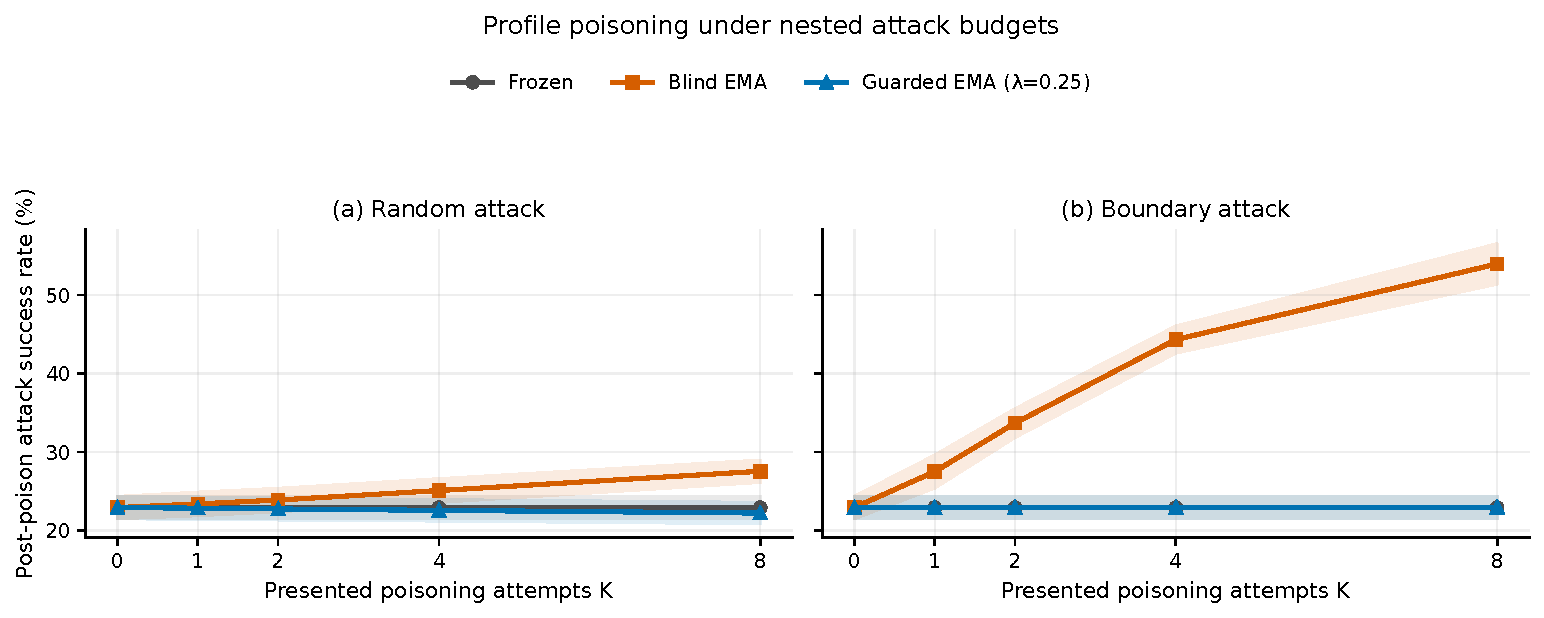
\includegraphics[width=\fulllength,height=0.73\textheight,keepaspectratio]{figures_revision_20261005/figure1_poisoning_asr.pdf}
\end{adjustwidth}
\caption{HMOG reference-point post-poison ASR on held-out impostor probes across nested numbers of presented poisoning attempts \(K\). Poison and probe source-session groups were disjoint, and the profile was frozen before probe evaluation. Lines are victim-macro fold summaries for Frozen, Blind EMA, and Guarded EMA (\(\lambda=0.25\)); shaded fold-level \(t\)-bands are descriptive because the five fitting partitions overlap. The paired victim-bootstrap interval for the primary boundary \(K=8\) contrast is reported in the text.\label{fig:reference-poisoning}}
\end{figure}

\subsection{Operating-point sensitivity, feasibility, and gate activity}\label{sec:operating-point-sensitivity-feasibility-and-gate-activity}

Nominal calibration targets did not determine held-out FAR (Table~\ref{tab:calibration-transfer}). Under the nominal-1\% condition, mean achieved calibration FAR was 0.91\% on HMOG and 0.79\% on McGill, whereas full-cohort held-out Frozen FAR was 1.04\% and 2.14\%. Full-cohort Frozen FRR was 80.79\% and 90.25\%, respectively. These values describe all structurally valid held-out paths and are not baselines for the conditional boundary effects.

\begin{table}[H]
\caption{Calibration and full-cohort held-out Frozen performance. Calibration values are unweighted means of claimant-profile pooled-observation rates. Held-out values use all structurally valid random-\(K=0\) paths with victim-macro aggregation. Nominal targets are calibration constraints, not held-out guarantees.\label{tab:calibration-transfer}}
\begin{adjustwidth}{-\extralength}{0cm}
\footnotesize
\setlength{\tabcolsep}{3.5pt}
\renewcommand{\arraystretch}{1.16}
\begin{tabularx}{\fulllength}{l L C C C L}
\toprule
\textbf{Dataset} & \textbf{Condition} & \textbf{Achieved calibration FAR} & \textbf{Full held-out Frozen FAR} & \textbf{Full held-out Frozen FRR} & \textbf{Cohort} \\
\midrule
HMOG & Reference (approximate EER) & 23.01\% & 22.92\% & 24.95\% & 500 calibration profiles; 100 held-out victims \\
HMOG & Nominal 5\% calibration FAR & 4.93\% & 5.07\% & 57.88\% & 500 calibration profiles; 100 held-out victims \\
HMOG & Nominal 1\% calibration FAR & 0.91\% & 1.04\% & 80.79\% & 500 calibration profiles; 100 held-out victims \\
McGill & Reference (minimum HTER) & 6.89\% & 12.20\% & 78.81\% & 20 calibration profiles; 20 held-out victims \\
McGill & Nominal 5\% calibration FAR & 3.66\% & 7.37\% & 82.43\% & 20 calibration profiles; 20 held-out victims \\
McGill & Nominal 1\% calibration FAR & 0.79\% & 2.14\% & 90.25\% & 20 calibration profiles; 20 held-out victims \\
\bottomrule
\end{tabularx}
\end{adjustwidth}
\end{table}

The boundary-\(K=8\) Blind-minus-Frozen effect decreased from +31.04 to +2.49 and then -0.447 points across HMOG reference, nominal-5\%, and nominal-1\% conditions (Table~\ref{tab:boundary-effects}; Figure~\ref{fig:operating-points}). McGill showed +19.72, +0.20, and -0.354 points; the nominal-5\% CI included zero. Guarded-minus-Blind was strongly negative at reference, smaller at nominal 5\%, and near zero at nominal 1\%. Cross-target rows are not strictly paired because recalibration changed \(\tau_0\), claimant-specific \(k\), selected candidates, and feasible paths.

\begin{table}[H]
\caption{Conditional boundary-\(K=8\) paired post-poison ASR effects. Each condition uses its own common feasible cohort and a 10,000-draw paired victim bootstrap. The reference rows use the sensitivity package's retained random streams; historical reference intervals remain in Section~\ref{sec:reference-poisoning} and the McGill corroboration. Three decimals preserve near-zero effects.\label{tab:boundary-effects}}
\begin{adjustwidth}{-\extralength}{0cm}
\footnotesize
\setlength{\tabcolsep}{2.6pt}
\renewcommand{\arraystretch}{1.18}
\begin{tabularx}{\fulllength}{l L L L c c c}
\toprule
\textbf{Dataset} & \textbf{Condition} & \textbf{Blind EMA -- Frozen ASR, pp [95\% CI]} & \textbf{Guarded EMA -- Blind EMA ASR, pp [95\% CI]} & \textbf{Eligible paths} & \textbf{Victims} & \textbf{Victim-fold units} \\
\midrule
HMOG & Reference & +31.04 [+26.97, +35.11] & -31.02 [-35.15, -26.98] & 49,889 / 50,000 & 100 & 500 \\
HMOG & Nominal 5\% & +2.49 [+0.95, +4.38] & -3.09 [-4.91, -1.61] & 49,753 / 50,000 & 100 & 500 \\
HMOG & Nominal 1\% & -0.447 [-0.502, -0.393] & -0.009 [-0.020, -0.001] & 9,088 / 50,000 & 100 & 302 \\
McGill & Reference & +19.72 [+5.50, +37.24] & -19.62 [-36.77, -5.66] & 1,456 / 2,000 & 18 & -- \\
McGill & Nominal 5\% & +0.20 [-0.05, +0.53] & -0.26 [-0.58, -0.03] & 1,369 / 2,000 & 18 & -- \\
McGill & Nominal 1\% & -0.354 [-0.552, -0.186] & 0.000 [0.000, 0.000] & 1,001 / 2,000 & 17 & -- \\
\bottomrule
\end{tabularx}
\end{adjustwidth}
\end{table}

\begin{figure}[H]
\begin{adjustwidth}{-\extralength}{0cm}
\centering
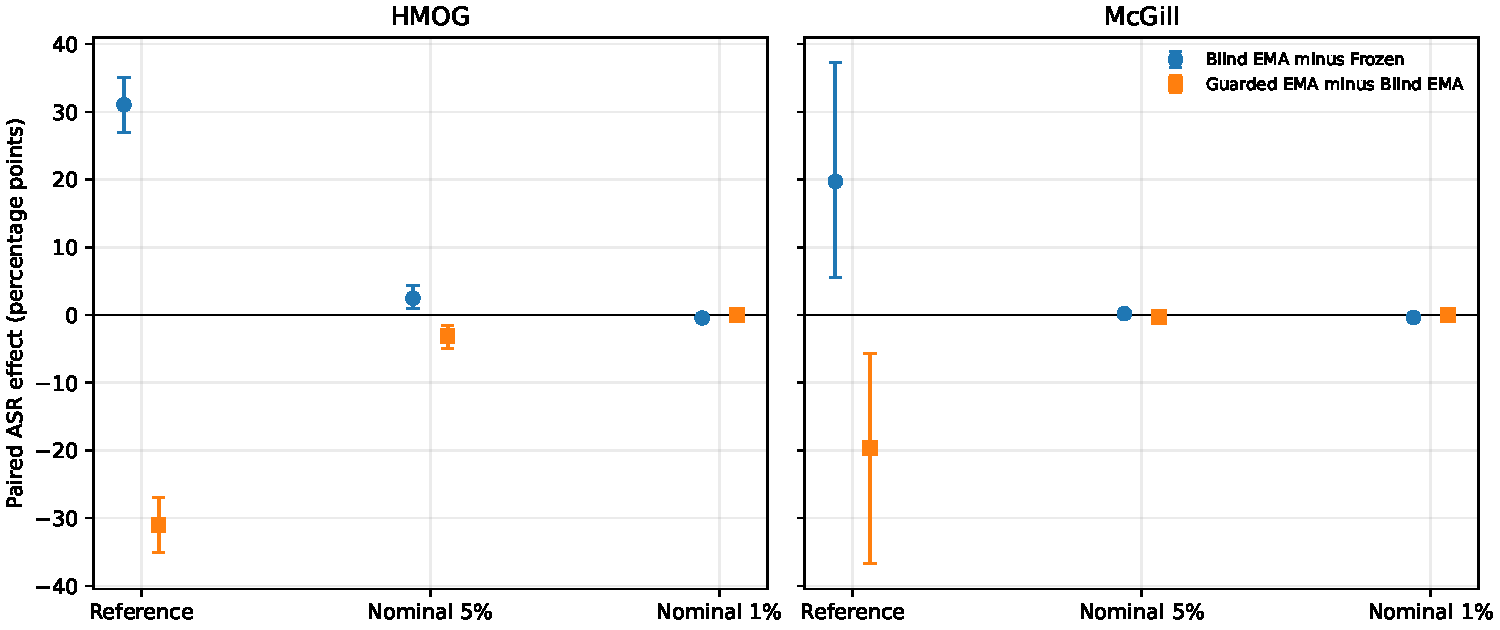
\includegraphics[width=\fulllength,height=0.73\textheight,keepaspectratio]{figures/figure2_boundary_k8_effects.pdf}
\end{adjustwidth}
\caption{Operating-point dependence of boundary-\(K=8\) post-poison ASR effects. Points are Blind EMA minus Frozen and Guarded EMA minus Blind EMA with paired victim-bootstrap 95\% intervals. Operating points are not connected because their feasible cohorts can differ. Source: frozen \texttt{boundary\_k8\_effects} artifact.\label{fig:operating-points}}
\end{figure}

For the sensitivity primary, a secondary victim-by-impostor-source bootstrap gave -0.447 points {[}\ensuremath{-}0.515, \ensuremath{-}0.383{]} for Blind minus Frozen and -0.009 points {[}\ensuremath{-}0.022, \ensuremath{-}0.001{]} for Guarded minus Blind. It covered 100 victims, 9,088 paths, and 100 observed impostor sources only in HMOG nominal 1\%, boundary \(K=8\); it did not add training or population uncertainty.

The negative strict-point ASR effect did not indicate harmless updating. On the same 9,088-path HMOG nominal-1\% cohort, Frozen ASR/\allowbreak FRR/\allowbreak HTER were 0.826\%/\allowbreak 80.18\%/\allowbreak 40.50\%, while Blind values were 0.379\%/\allowbreak 87.07\%/\allowbreak 43.73\%. Blind increased FRR by 6.89 points (95\% CI {[}+5.63, +8.27{]}) and HTER by 3.22 points (95\% CI {[}+2.59, +3.91{]}). The experiment did not specify a separate availability-oriented attacker, so this result is not presented as a demonstrated denial-of-service attack.

Strict calibration also reduced feasibility. HMOG nominal 1\% retained 9,088 of 50,000 planned boundary paths across 100 victims and 302 of 500 victim-fold units; McGill retained 1,001 of 2,000 paths across 17 victims. Excluded paths lacked eight initially accepted candidates and were not assigned zero ASR. At this condition the Guarded gate exceeded authentication in 19.22\% of 72,704 HMOG poisoning states and 13.49\% of 8,008 McGill states. Initial \(k<0\) occurred in 443 of all 500 HMOG claimant-fold profiles and 15 of all 20 McGill profiles, a different denominator. The sign of \(k\) alone does not explain the aggregate reversal. On McGill nominal 1\%, Blind and Guarded had equal aggregate ASR but MURs of 69.36\% and 62.32\%; equal endpoints did not imply equal updates or trajectories.

The gate percentages are state-weighted diagnostics, while the paired ASR effects are victim-macro estimates and the negative-\(k\) values use all calibration profiles. They are presented together to describe the mechanism but should not be read as interchangeable sampling units.

\subsection{Clean temporal behavior and Oracle diagnostic}\label{sec:clean-temporal-behavior-and-oracle-diagnostic}

Under the primary claimant-only HMOG synthetic shift at \(D=2\), Frozen late FRR/\allowbreak FAR/\allowbreak HTER were 32.53\%/\allowbreak 22.86\%/\allowbreak 27.70\%. Guarded values were 34.60\%/\allowbreak 21.73\%/\allowbreak 28.16\%, corresponding to a late-FRR gain of -2.07 points (95\% CI {[}-3.53, -0.63{]}) relative to Frozen. Blind late FRR was 32.20\%, with a gain of +0.33 points (95\% CI {[}-1.20, +1.93{]}). Neither accepted-only method showed a clear improvement in the prespecified late-FRR endpoint (Figure~\ref{fig:temporal-tradeoff}).

Blind late FAR changed by +0.93 points (95\% CI {[}-0.58, +2.64{]}) and its HTER gain was -0.30 points (95\% CI {[}-1.02, +0.40{]}). Guarded late FAR changed by -1.14 points (95\% CI {[}-2.29, +0.12{]}), while its HTER gain was -0.46 points (95\% CI {[}-1.16, +0.21{]}). Guarded's lower FAR point estimate was accompanied by higher FRR rather than a free improvement.

Oracle-all made every ground-truth genuine adaptation candidate update-eligible. At \(D=2\), its late-FRR gain over Frozen was +6.60 points (95\% CI {[}+4.90, +8.40{]}), accompanied by a +6.08-point late-FAR change (95\% CI {[}+4.20, +8.16{]}). At \(D=0\), it already lowered late FRR by 4.73 points and raised late FAR by 5.51 points. Its result therefore reflects operating-point movement as well as response to synthetic shift. Guarded mean and threshold moved upward across the five retained checkpoints, while the Oracle-all state moved downward; Guarded update rate fell from 63.47\% to 51.68\%, and Oracle-all update eligibility remained 100\% (Figure~\ref{fig:profile-trajectories}).

Oracle-all HTER gains relative to Frozen were -0.39, -0.28, and +0.26 points at \(D=0,1,2\), and all three CIs included zero. The opposing FRR and FAR changes therefore produced little balanced-error improvement. Complete intermediate-level effects are reported in Supplementary Results S5.

\begin{figure}[H]
\centering
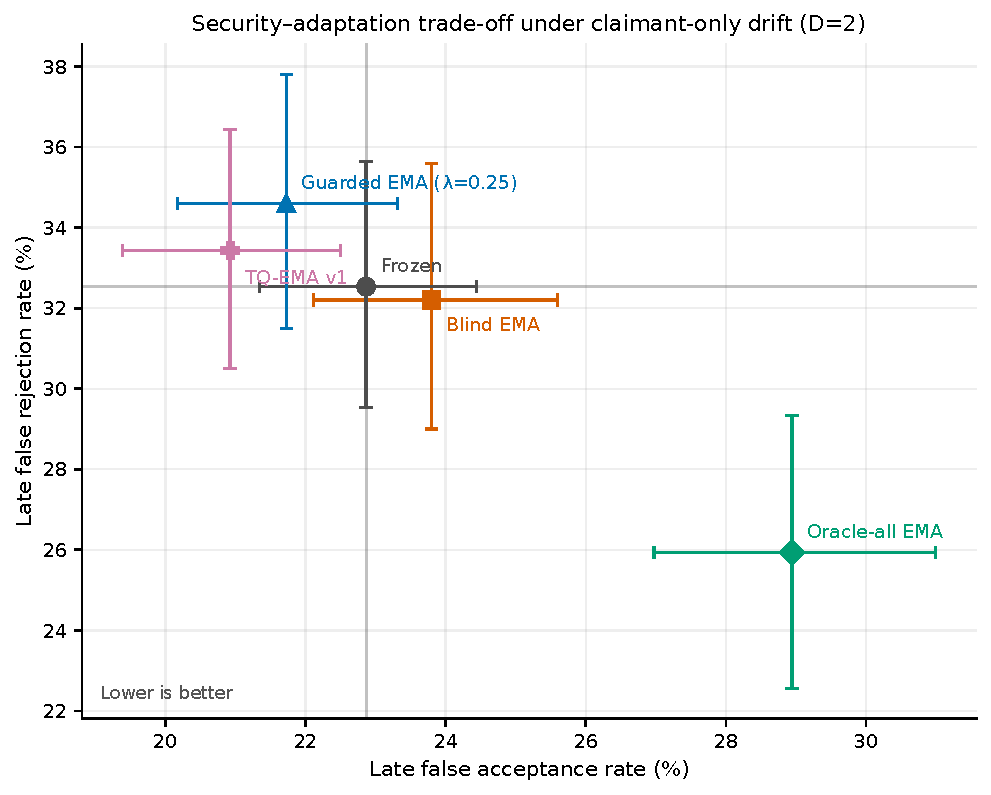
\includegraphics[width=0.92\textwidth,height=0.70\textheight,keepaspectratio]{figures/figure3_security_adaptation_tradeoff.pdf}
\caption{HMOG late FAR-FRR operating points under claimant-only synthetic shift \(D=2\). Points are subject-macro estimates for Frozen, Blind EMA, Guarded EMA (\(\lambda=0.25\)), Oracle-all, and TQ-EMA v1. Bars are 95\% subject-bootstrap percentile intervals for each method's absolute late FAR (horizontal) and late FRR (vertical), after subject-level fold aggregation; paired intervals for between-method differences are reported in the text. Lower values on both axes are preferable.\label{fig:temporal-tradeoff}}
\end{figure}

\begin{figure}[H]
\begin{adjustwidth}{-\extralength}{0cm}
\centering
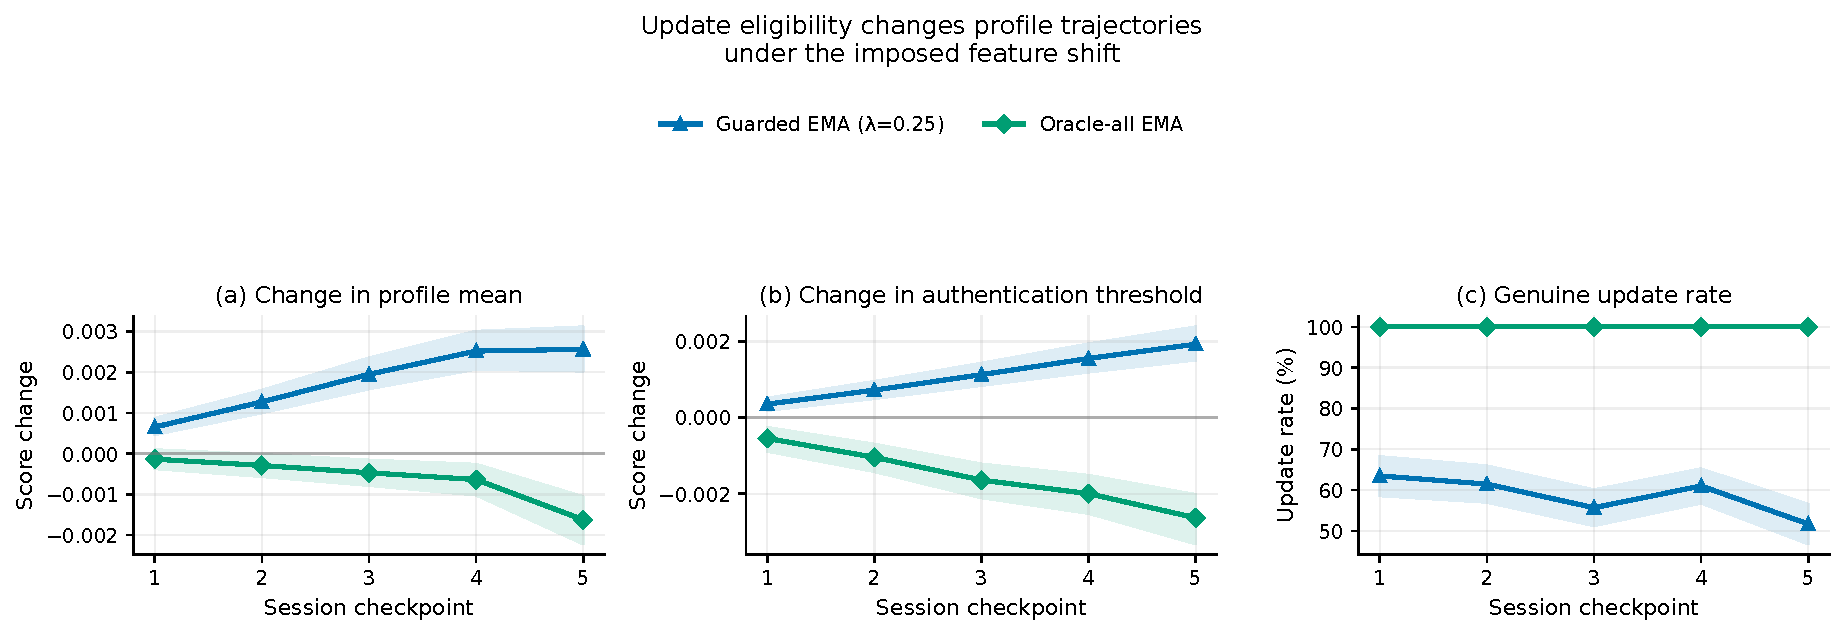
\includegraphics[width=\fulllength,height=0.73\textheight,keepaspectratio]{figures_revision_20261005/figure4_selection_bias_mechanism.pdf}
\end{adjustwidth}
\caption{HMOG profile trajectories under claimant-only synthetic shift \(D=2\). Panels show change from enrollment in profile mean and authentication threshold, plus genuine update rate, across five evaluation checkpoints for Guarded EMA and Oracle-all. Lines are subject-level means and bands are subject-bootstrap 95\% intervals. Oracle-all is label-aware and non-deployable.\label{fig:profile-trajectories}}
\end{figure}

\subsection{McGill cross-day corroboration}\label{sec:mcgill-cross-day-corroboration}

The frozen Day-1 McGill classifier attained 58.12\% validation top-1 accuracy and passed its prespecified 20\% viability gate before Day-2 scores were loaded. At reference boundary \(K=8\), ASR was 12.37\% for Frozen, 32.09\% for Blind, and 12.48\% for Guarded (Table~\ref{tab:mcgill-results}). The paired Blind-minus-Frozen effect was +19.72 points (historical 95\% CI {[}+5.58, +37.34{]}); Guarded-minus-Blind was -19.62 points (95\% CI {[}-37.17, -5.60{]}). Blind MUR was 100\%, and Guarded MUR was 32.22\%. The eligible cohort contained 1,456 of 2,000 paths across 18 victims; 544 paths lacked eight accepted candidates. The random-\(K=8\) Blind effect was +1.51 points across all 20 subjects, with a CI {[}-0.09, +4.43{]} that included zero.

In the Day-2 temporal stream, Guarded late FRR was 81.00\% versus 78.00\% for Frozen, while Oracle-all FRR was 12.75\%. Oracle-all FAR reached 75.05\%, compared with 11.46\% for Frozen and 10.29\% for Guarded. The results reproduce the reference-point directions under a difficult cross-day setting but do not establish comparable absolute performance or isolate behavioral drift. Frozen McGill figures are retained in Supplementary Results S6.

The McGill implementation used the actual unclipped decision threshold \(\mu-k\sigma\). The subject-macro Oracle-all threshold in Figure S6 became negative because individual Oracle-all profiles were permitted to move below zero under that executed rule. The plotted line averages saved individual thresholds after each adaptation step; it is not reconstructed from aggregated moments. No clipped counterfactual was run, and the McGill results are interpreted under this documented dataset-specific policy.

Guarded-minus-Frozen late FRR was +3.00 points (95\% CI {[}0.00, +7.00{]}). Oracle-all-minus-Frozen FRR was -65.25 points (95\% CI {[}-83.75, -45.50{]}), while Oracle-all-minus-Guarded FAR was +64.76 points (95\% CI {[}+48.93, +79.24{]}). These large opposing changes explain why the three late HTER values were much closer than their separate FAR and FRR components.

\begin{table}[H]
\caption{McGill reference poisoning and cross-day temporal evidence. Poisoning effects average repeats within victims before paired subject bootstrap. Temporal endpoints are subject-macro rates over the last 20 of 80 adaptation-checkpoint pairs. Oracle-all uses labels only for update eligibility and is not deployable.\label{tab:mcgill-results}}
\begin{adjustwidth}{-\extralength}{0cm}
\footnotesize
\setlength{\tabcolsep}{2.5pt}
\renewcommand{\arraystretch}{1.2}
\begin{tabularx}{\fulllength}{L L C C C C L}
\toprule
\textbf{McGill analysis} & \textbf{Cohort} & \textbf{Frozen} & \textbf{Blind EMA} & \textbf{Guarded EMA} & \textbf{Oracle-all} & \textbf{Paired effect [95\% CI], pp} \\
\midrule
Reference boundary \(K=8\), post-ASR & 1,456 paths; 18 victims & 12.37\% & 32.09\% & 12.48\% & -- & Blind -- Frozen: +19.72 [+5.58, +37.34] \\
Day-2 late FRR / FAR / HTER & 20 subjects & 78.00 / 11.46 / 44.73\% & -- & 81.00 / 10.29 / 45.64\% & 12.75 / 75.05 / 43.90\% & Guarded -- Frozen FRR: +3.00 [0.00, +7.00] \\
\bottomrule
\end{tabularx}
\end{adjustwidth}
\end{table}

\subsection{Supporting recovery and state probes}\label{sec:supporting-recovery-and-state-probes}

TQ-EMA v1 reached outer evaluation but did not meet its recovery criterion. In claimant-only \(D=2\), late-FRR gain was -0.90 points (95\% CI {[}-1.80, 0.00{]}); late FAR changed by -1.94 points, and HTER gain was +0.52 points. The event audit recorded 1,404 trusted and 49 recovery updates. TQ-EMA v2 then failed its validation gate because fold 4 had no configuration satisfying both safety constraints. No Adaptive Quantile setting was feasible in all folds. The latter branches have \texttt{outer\_test\_loaded=false} and no outer estimates. Their complete specifications and validation outcomes appear in Supplementary Methods S6-S10 and Supplementary Results S1-S3.

TQ-v1's complete-five-fold sensitivity did not reverse the stopping decision. TQ-v2 had feasible selections in four folds, but all selected late-FRR gains were negative; fold 4 triggered the fail-closed rule. These validation values are documented in the Supplement and are not presented as outer performance.

\section{Discussion}\label{sec:discussion}

\subsection{Coupled feedback effects and operating-point scope}\label{sec:coupled-feedback-effects-and-operating-point-scope}

Accepted-only updating linked two forms of evidence selection in the evaluated systems. An accepted impostor could enter the profile and alter later decisions, while a rejected claimant observation could not inform adaptation. At the reference operating points, the first pathway produced large Blind-minus-Frozen ASR increases on HMOG and McGill. The sensitivity analysis set an important boundary around this result. Amplification was much smaller at nominal 5\%, the McGill interval included zero, and the mean effect was negative at nominal 1\% for the tested boundary strategy.

Poison and probe observations were separated before selection, and state was frozen before future probes were scored. The reference increase therefore concerns acceptance of unused impostor observations after profile change. During the malicious-only phase, the blocking Oracle retained Frozen's state and outcomes, while Blind could update. This matched control supports profile modification as the experimental difference at reference without extending the result to every attacker or operating point.

The reversal cannot be attributed to threshold movement alone. For a permitted update exactly on the current unclipped boundary, the local EMA identity in Section 3.3 predicts opposite threshold directions for positive and negative \(k\). The experiment is more complex: recalibration changed the initial threshold and its associated \(k\), then changed which boundary samples were selected and which paths contained eight eligible candidates. Candidates were ranked around the initial rather than evolving boundary, margins were nonzero, Guarded could reject updates, and cohorts differed. Negative \(k\) was common at nominal 1\%, but its sign does not determine an eight-step aggregate endpoint. Candidate ranking was not re-optimized for all possible strict-point adversaries. The sensitivity results therefore describe recalibrated policies and their condition-specific feasible paths.

A smaller ASR effect also did not imply benign state change. On the matched HMOG nominal-1\% cohort, Blind reduced future impostor acceptance but increased FRR and HTER. This genuine-rejection cost was observed under an integrity-oriented boundary attack; the experiment did not design or test a separate denial-of-service objective. Full-cohort held-out FAR, conditional boundary ASR, calibration FRR, and clean-temporal FRR remain distinct endpoints. The strict calibration conditions also had high full-cohort FRR, limiting their practical interpretation.

HTER is useful for summarizing balanced error, but opposing FAR and FRR movements can leave it nearly unchanged while altering operational risk. Security and usability costs are not necessarily symmetric. The separate endpoints in this study are therefore more informative than selecting a method from HTER alone.

\subsection{State-dependent update authorization}\label{sec:state-dependent-update-authorization}

Guarded EMA tested a known design principle: access permission and update eligibility can use different criteria. Its reference-point results show that this intervention can suppress additional contamination under the studied state. The effective added margin was \(\lambda\max(\mu_{\mathrm{enroll}}-\tau_{\mathrm{auth}},0)\), so it disappeared whenever the authentication threshold reached or exceeded the enrollment mean. This state was common after nominal-1\% recalibration, and the additional Guarded ASR effect became very small.

The common access-rule form should not be confused with common realized decisions. Blind and Guarded acquire different update histories, which can produce different later means, thresholds, and accept/reject outcomes. The same distinction applies when an aggregate endpoint coincides. McGill nominal-1\% Blind and Guarded ASR estimates were equal, but their MURs differed. MUR is itself incomplete because update identity and state displacement affect later outcomes as well as the number incorporated.

The Guarded result supports auditing an authorization rule over its reachable state space. A separately named update threshold may supply no extra restriction in some states, and stronger gating may remove legitimate update opportunities. The exploratory lambda sweep illustrated this trade-off but did not identify a universally optimal value.

\subsection{Oracle and recovery probes}\label{sec:oracle-and-recovery-probes}

The clean temporal controls examined the other side of accepted-only feedback. Under the claimant-only synthetic shift, Guarded retained a higher-scoring subset of genuine candidates and its mean and threshold moved upward. Oracle-all made rejected genuine candidates update-eligible and produced a downward trajectory with lower FRR and higher FAR. These patterns support feedback availability as one contributor to weak recovery. Oracle-all retains the authentication rule form, but its altered state can change subsequent thresholds and decisions.

Oracle-all does not define a secure or optimal trajectory. It requires ground-truth labels during operation, and its FAR increase offset much of the FRR improvement. It also changes both the composition of update observations and the number and frequency of permitted updates; the present comparison does not isolate these factors with a count-matched control. The same direction was already visible at \(D=0\), showing that the contrast includes ordinary operating-point movement rather than only recovery from synthetic shift. The fold-specific feature perturbation also passed through a nonlinear score model; it did not guarantee an identical downward score displacement for every subject.

The recovery probes did not resolve this trade-off within their frozen designs and short replay. TQ-EMA v1 admitted temporally consistent rejected evidence but applied only 49 recovery updates against 1,404 trusted updates and did not improve late FRR. TQ-EMA v2 addressed this imbalance but failed the validation gate, and the Quantile branch had no feasible setting in any fold. These outcomes apply to the specified controllers, grids, constraints, and horizon. They do not establish that quarantine or distributional tracking cannot recover over longer streams, and no outer claim is available for the validation-stopped branches.

\subsection{External corroboration and practical implications}\label{sec:external-corroboration-and-practical-implications}

McGill changed the dataset, classifier, modalities, temporal split, and threshold implementation. The reference-point Blind amplification, Guarded suppression, and Oracle trajectory direction recurred under McGill's documented unclipped \(\mu-k\sigma\) policy, which strengthens the bounded mechanism interpretation but is not an algorithm-identical replication of HMOG's zero-clipped threshold. The small cohort and severe Day-2 degradation limit effect-size generalization. Day separation can combine behavior, activity, placement, acquisition, and model-transfer changes; it is not an isolated measure of natural behavioral drift.

The attacker model also constrains application. Boundary selection assumed access to claimant scores and a pool large enough to screen initially accepted samples. \(K\) counted presented poisons after this screening. Deployments that hide scores, limit queries, or aggregate decisions differently may change both feasibility and effect. The nominal-1\% exclusions already show that an operating point can alter which attack paths enter the conditional estimate.

Calibration transfer creates a related deployment issue. A nominal constraint estimated on validation or Day-1 enrollment data did not guarantee the same held-out FAR, especially under McGill's cross-day shift. Tightening calibration also increased genuine rejection and reduced the set of feasible boundary paths. Reporting the target without these held-out and feasibility outcomes would conceal the population on which the attack estimate is conditional.

For similar systems, security and adaptation should be assessed through multiple endpoints at stated operating points. Post-update ASR or FAR should be accompanied by FRR, update composition, calibration transfer, gate activity, and attack feasibility. Recovery evidence partly independent of the current biometric threshold, such as verified step-up authentication or temporally separated corroboration, may help escape accepted-only censoring. Such evidence would still require bounded and auditable state changes.

The results also separate mechanism corroboration from benchmark comparison. McGill was not used to rank its classifier against the HMOG model: the subject set, input channels, windowing, calibration data, and temporal split all differed. Its value is that the same directional relationships recurred under a protocol fixed before Day-2 access. Absolute FAR, FRR, and ASR differences between datasets should therefore not be attributed to one method component.

Update rate alone is insufficient as a security outcome. Guarded incorporated a larger malicious fraction on McGill than on HMOG at reference, yet both post-poison ASR estimates remained close to their corresponding Frozen baselines. State displacement depends on which observations are admitted and on the current profile, not only on the count. Evaluation should therefore retain MUR together with threshold, location, and scale changes.

\subsection{Limitations and future directions}\label{sec:limitations-and-future-directions}

The main HMOG temporal evidence used synthetic standardized-feature shifts whose magnitudes were not calibrated to natural change. Numeric session identifiers defined the replay order, but the available source does not independently validate them as a behavioral chronology. Each eligible victim-fold replay contained only four or five adaptation opportunities, so conclusions concern late FRR within that short horizon rather than long-term recovery. The initial 500-sample truncation also lacks a documented scientific rationale in the inherited source. HMOG methods were developed sequentially on previously inspected outer caches. The operating-point analysis was prospectively specified, but it reused those caches and is a sensitivity study rather than untouched confirmation.

The five HMOG folds share fitting data, and victim-bootstrap intervals condition on fixed models and observed pools. Within the poisoning operating-point analysis, source-level resampling was retained only for HMOG nominal 1\%, boundary \(K=8\); source-resolved outcomes were unavailable for the historical reference poisoning package. A separate TQ-v1 clean-temporal analysis resampled victim and impostor-source identities for late FAR. Neither analysis covers training variation or a broader deployment population, and the poisoning analysis does not cover McGill. McGill contributed 20 subjects, with 17 or 18 in strict or reference boundary cohorts. The study considered score-profile adaptation from fixed LSTMs and did not evaluate feature or classifier updating, a binary-feedback boundary search, combined drift-plus-attack recovery, or broader attacks such as replay and sensor injection.

The two datasets also cover a narrow range of activities, devices, and sensing configurations. HMOG supplied the detailed mechanism study, while McGill used accelerometer-only inputs and showed severe Day-2 degradation. Agreement in direction at the reference point is useful corroboration, but it does not estimate population-level effect stability or establish acceptable authentication performance.

All online policies acted on cached scores from fixed classifiers. This design isolates score-profile updating and permits exact pairing, but it leaves interactions with representation learning, sensor adaptation, and model retraining unresolved. The reported intervals also condition on those fitted classifiers. They quantify variation over the retained victims and protocol randomization, not uncertainty from refitting the score generator on another sample.

The boundary and temporal studies were also separate. TQ-v1 was not tested in a combined drift-plus-poisoning stream, and the stopped branches supplied no outer evidence. The manuscript consequently supports a joint evaluation requirement, not a claim that one tested policy satisfies both security and recovery objectives.

No production deployment measured latency, memory, energy, step-up frequency, or user burden. Larger multi-day studies should retain natural chronology, support victim- and impostor-source uncertainty, and evaluate legitimate change together with adversarial contamination. Future methods could test independently trusted recovery evidence or richer adaptive representations under parameters fixed before outer evaluation.

Within project BR28713099, future work may examine how trustworthy continuous-authentication evidence can support secure personalized credit services intended to strengthen citizens' financial resilience and reduce economic inequality.

The tested state was limited to scalar score location and scale. Feature normalization, embedding adaptation, uncertainty-aware state models, or explicit change detection may respond differently, but they would inherit the same need for trusted update evidence and held-out adversarial evaluation. Field studies should also report how often recovery invokes explicit authentication and whether rollback or rate limits create unacceptable friction.

\section{Conclusion}\label{sec:conclusion}

Accepted-only online adaptation couples access decisions to the evidence available for future learning. Prior biometric work established erroneous impostor inclusion, genuine-update misses, and separate update thresholds; this study evaluated their coupled consequences in paired fixed-score mobile-authentication protocols. At the historical reference operating points, score-informed boundary poisoning produced large Blind EMA increases in held-out attack success on HMOG and McGill. Guarded EMA used a separate update-authorization condition and kept the reference-point aggregate ASR close to Frozen.

These effects were not invariant under recalibration. Blind amplification narrowed at nominal 5\%, and its mean nominal-1\% effect was negative on both datasets for the tested boundary strategy. On the matched strict HMOG cohort, however, Blind increased FRR by 6.89 percentage points and HTER by 3.22 points. Lower attack success therefore did not establish harmless updating or general poisoning resistance. Recalibration changed the initial threshold, its associated \(k\), boundary candidates, and feasible paths. The Guarded margin was also state dependent: it added no restriction when the authentication threshold reached or exceeded the enrollment mean.

The temporal experiments provided no deployable recovery solution within the evaluated horizons. Guarded did not improve the primary late-FRR endpoint in the short HMOG replay, while label-aware Oracle-all changed both update composition and update frequency, lowered FRR, and raised FAR. TQ-EMA v1 missed its recovery criterion, and TQ-EMA v2 and Quantile stopped at validation without outer estimates. Under these protocols, adaptive authentication should be evaluated through joint reporting of post-update ASR or FAR, FRR, calibration transfer, update composition, gate activity, and attack feasibility. The findings motivate testing bounded recovery mechanisms that obtain trusted evidence partly independently of the current access decision.


% Only the existence and contents of the Supplement are confirmed at assembly time.
% Every remaining declaration requires explicit author confirmation before submission.
\supplementary{The separate Supplementary Materials file contains Supplementary Methods S1--S10, Supplementary Results S1--S6, Tables S1--S4, and Figures S1--S6.}

\authorcontributions{\textit{Author confirmation pending.}}

\funding{\textit{Author confirmation pending.}}

\institutionalreview{\textit{Author confirmation pending.}}

\informedconsent{\textit{Author confirmation pending.}}

\dataavailability{The study used the HMOG and McGill Gait datasets under the original providers' access terms; raw data are not redistributed with this package. The code and derived-results repository is private at the time of this working draft, and no public archive or DOI has been assigned. The final access route requires author confirmation before submission.}

\acknowledgments{\textit{Author confirmation pending, including any disclosure required for AI-assisted tools used in the current workflow.}}

\conflictsofinterest{\textit{Author confirmation pending.}}


\begin{adjustwidth}{-\extralength}{0cm}
\reftitle{References}
\bibliography{references_mdpi}
\end{adjustwidth}

\end{document}
